\chapter{Future Work \& Planning}
\label{cha:planning}
\section{Intro}
\label{sec:planningIntro}
The initial stage of this project focused on 
studying and understanding the problem,
analyzing existing \gls{eRange} solutions.
From then, researching usable a \gls{dataset}
was prioritized as it would prove vital
for testing the study's model.
Settling in two equally valid \glspl{dataset}
(\cite{vedDataset} and \cite{emobpy}),
the new focus for this study shifted on
implementing an existing solution of 
the "basic", and adaptive history based model
approaches (proposed by \cite{classicEVX})
while also writing this report and thus,
additional research on existing related works 
was conducted for better understanding
of the problem regarding \gls{eRange} estimation
and its difficulties.

\section{Planning}
\label{sec:planningPlanning}

\begin{figure}[H]
    \begin{center}
        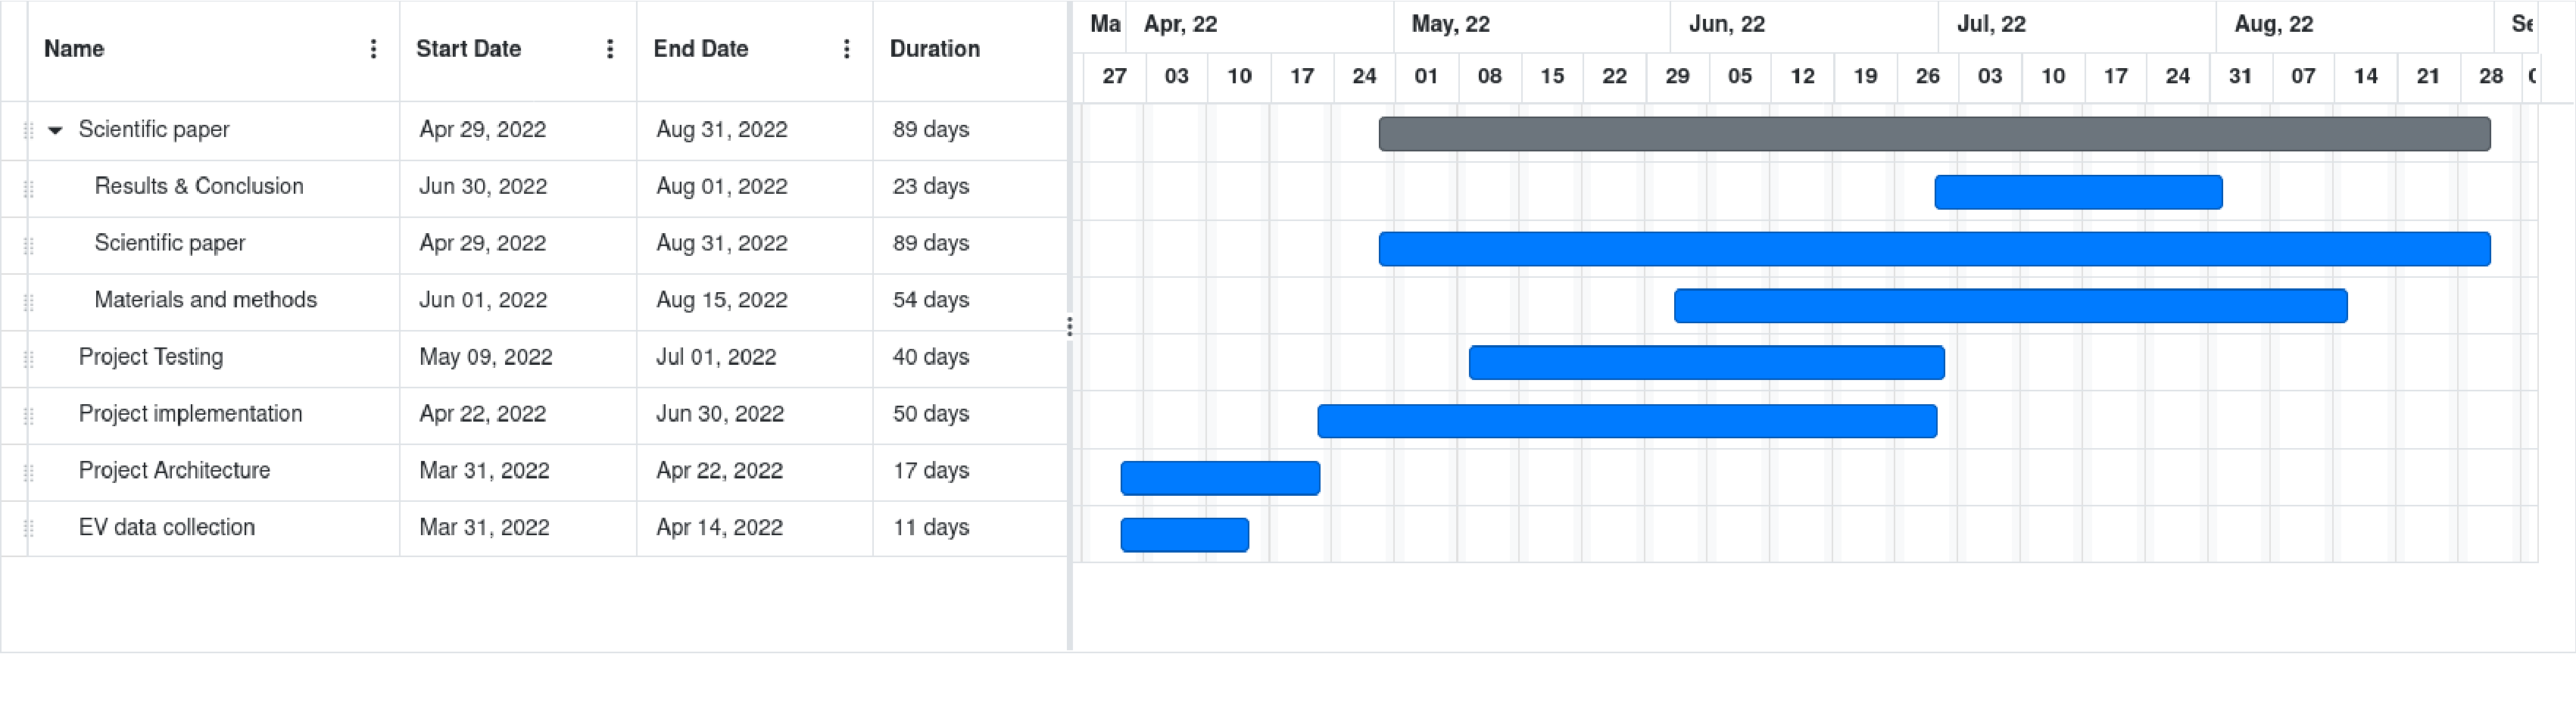
\includegraphics[scale=0.27]{../figures/planning}
        \caption{Project planning.}
    \end{center}
\end{figure}

\todo[inline]{Explicar principais tarefas}
\todo[inline]{Explicar dependencias de tarefas}
\todo[inline]{Quais os riscos}